\begin{frame}{LoRaWAN: Do It Yourself (DIY) Enddevice -- My current Prototype}
\begin{columns}
    \begin{column}{0.6\linewidth}
        \begin{center}
            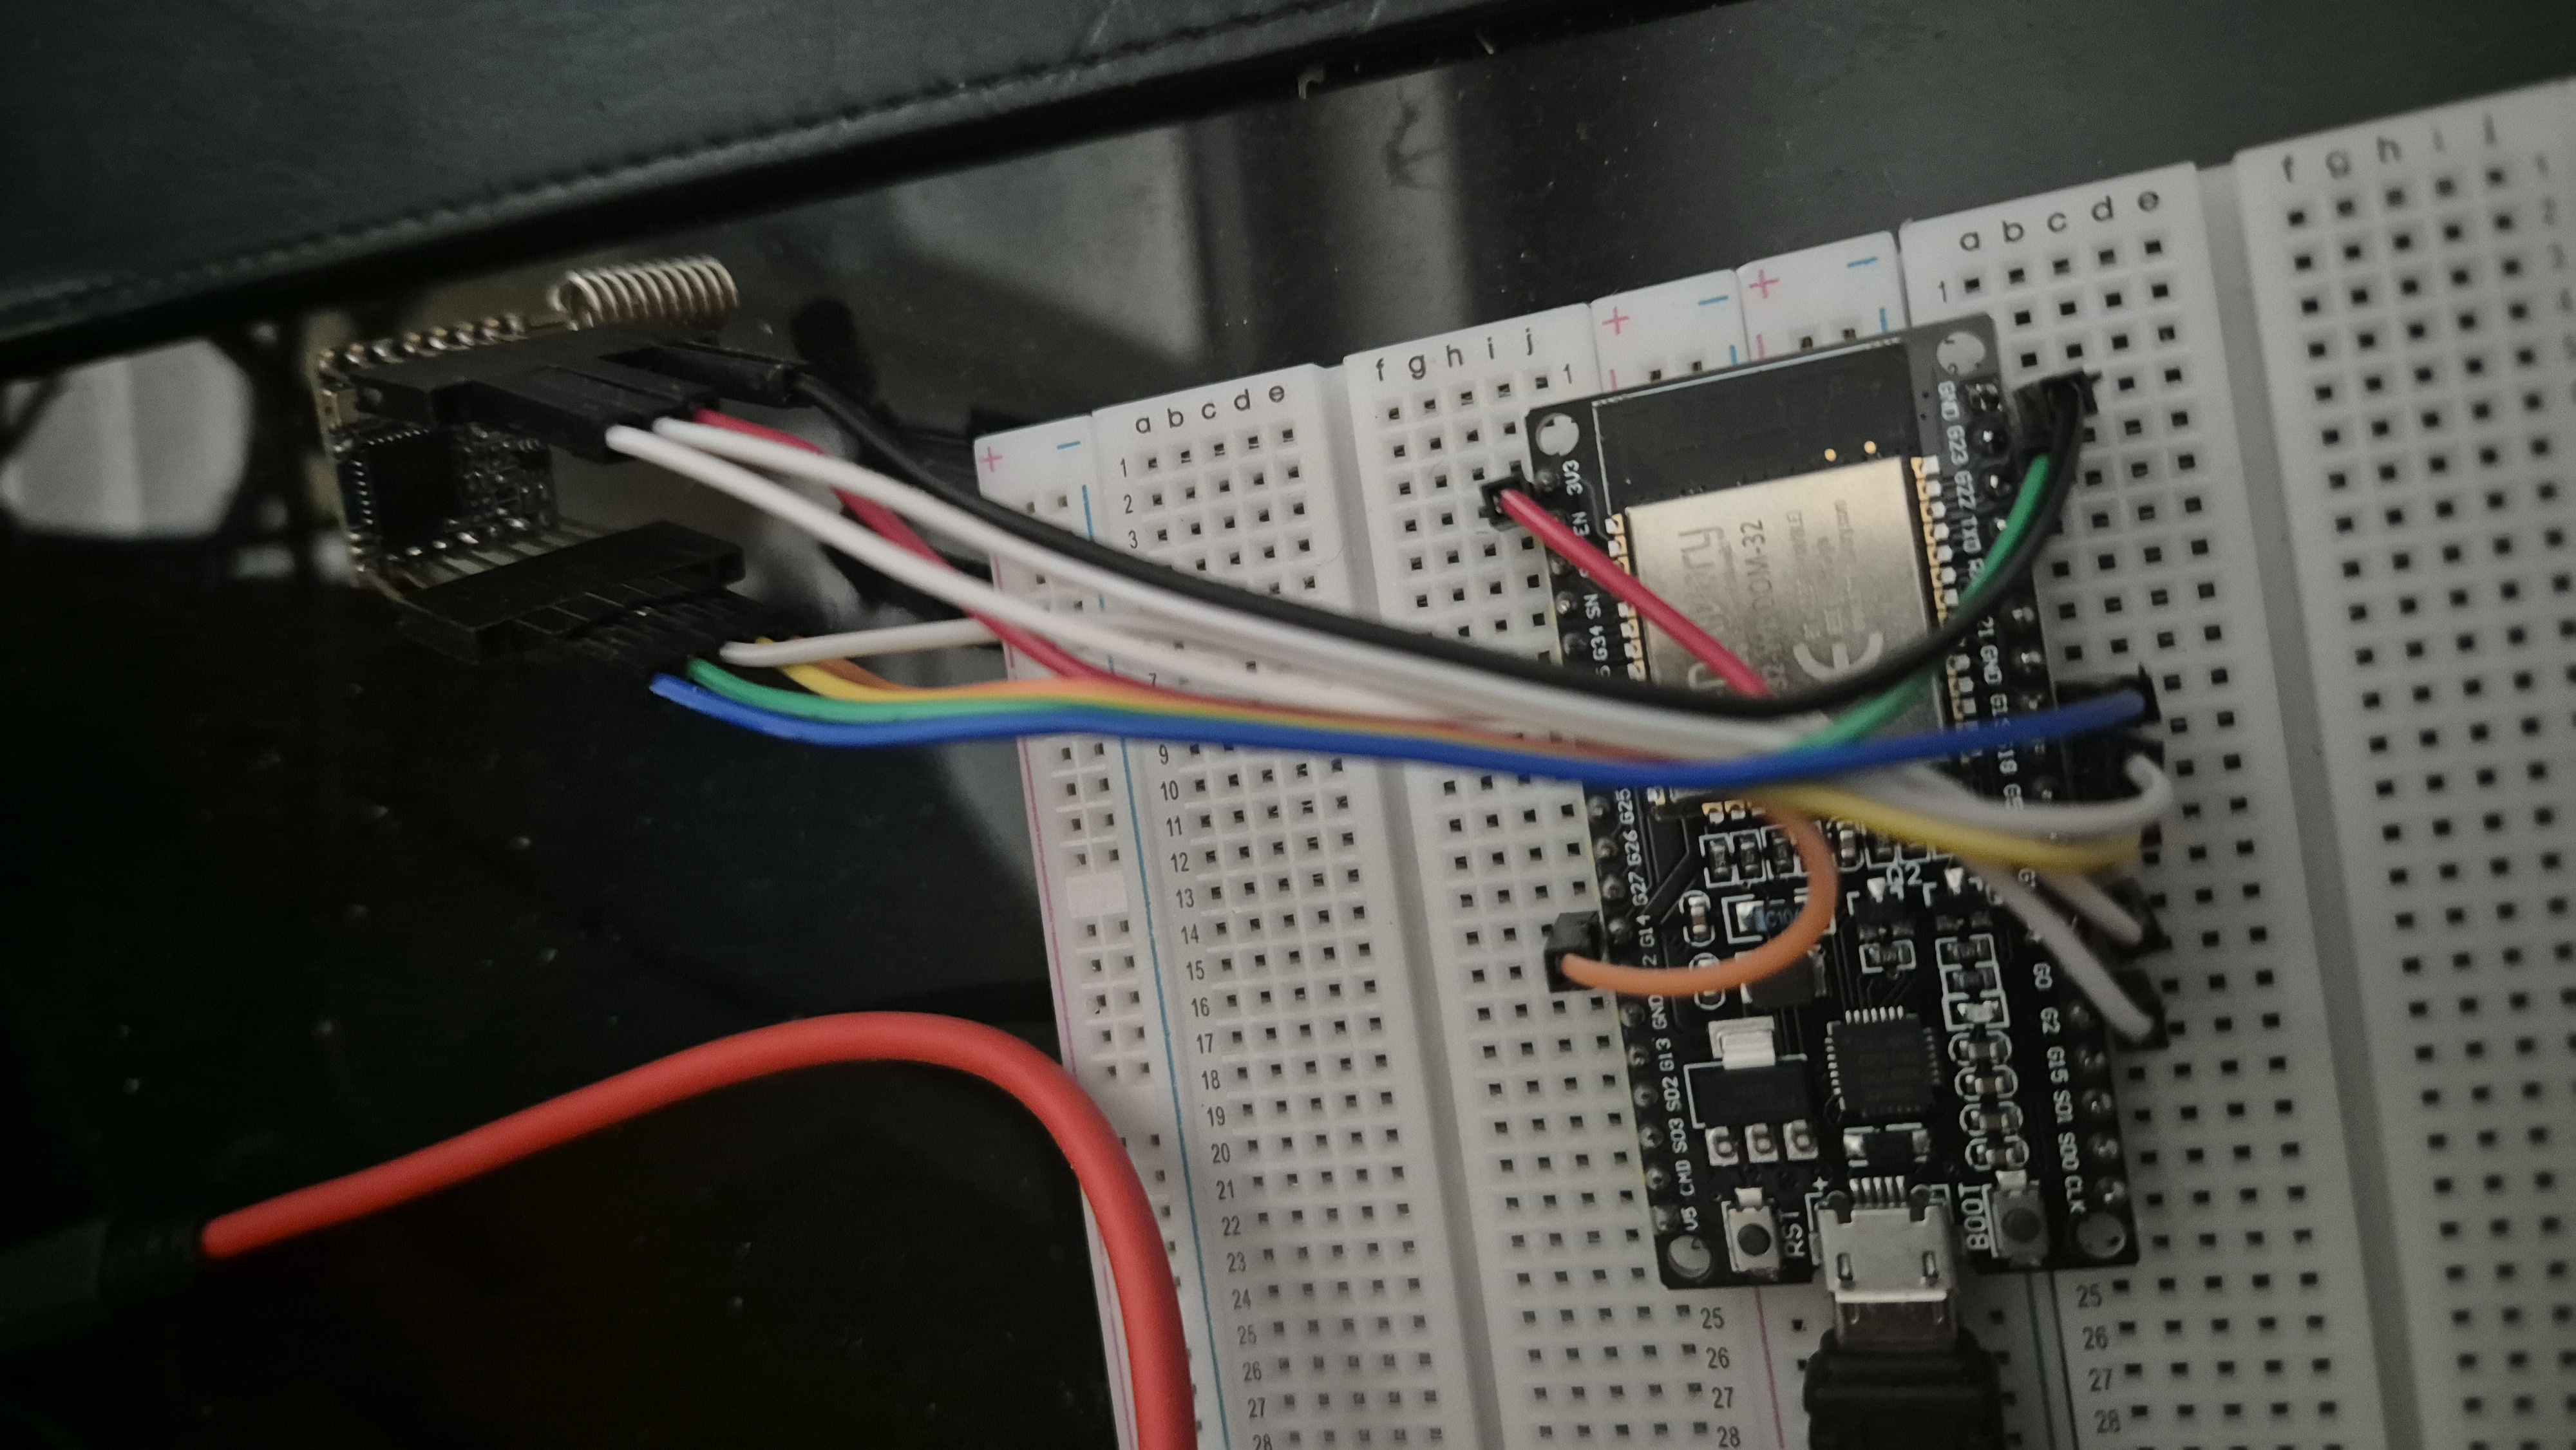
\includegraphics[width=1\textwidth]{material/enddevice-prototype.jpg}
        \end{center}
    \end{column}
    \begin{column}{0.4\linewidth}
        \begin{center}
            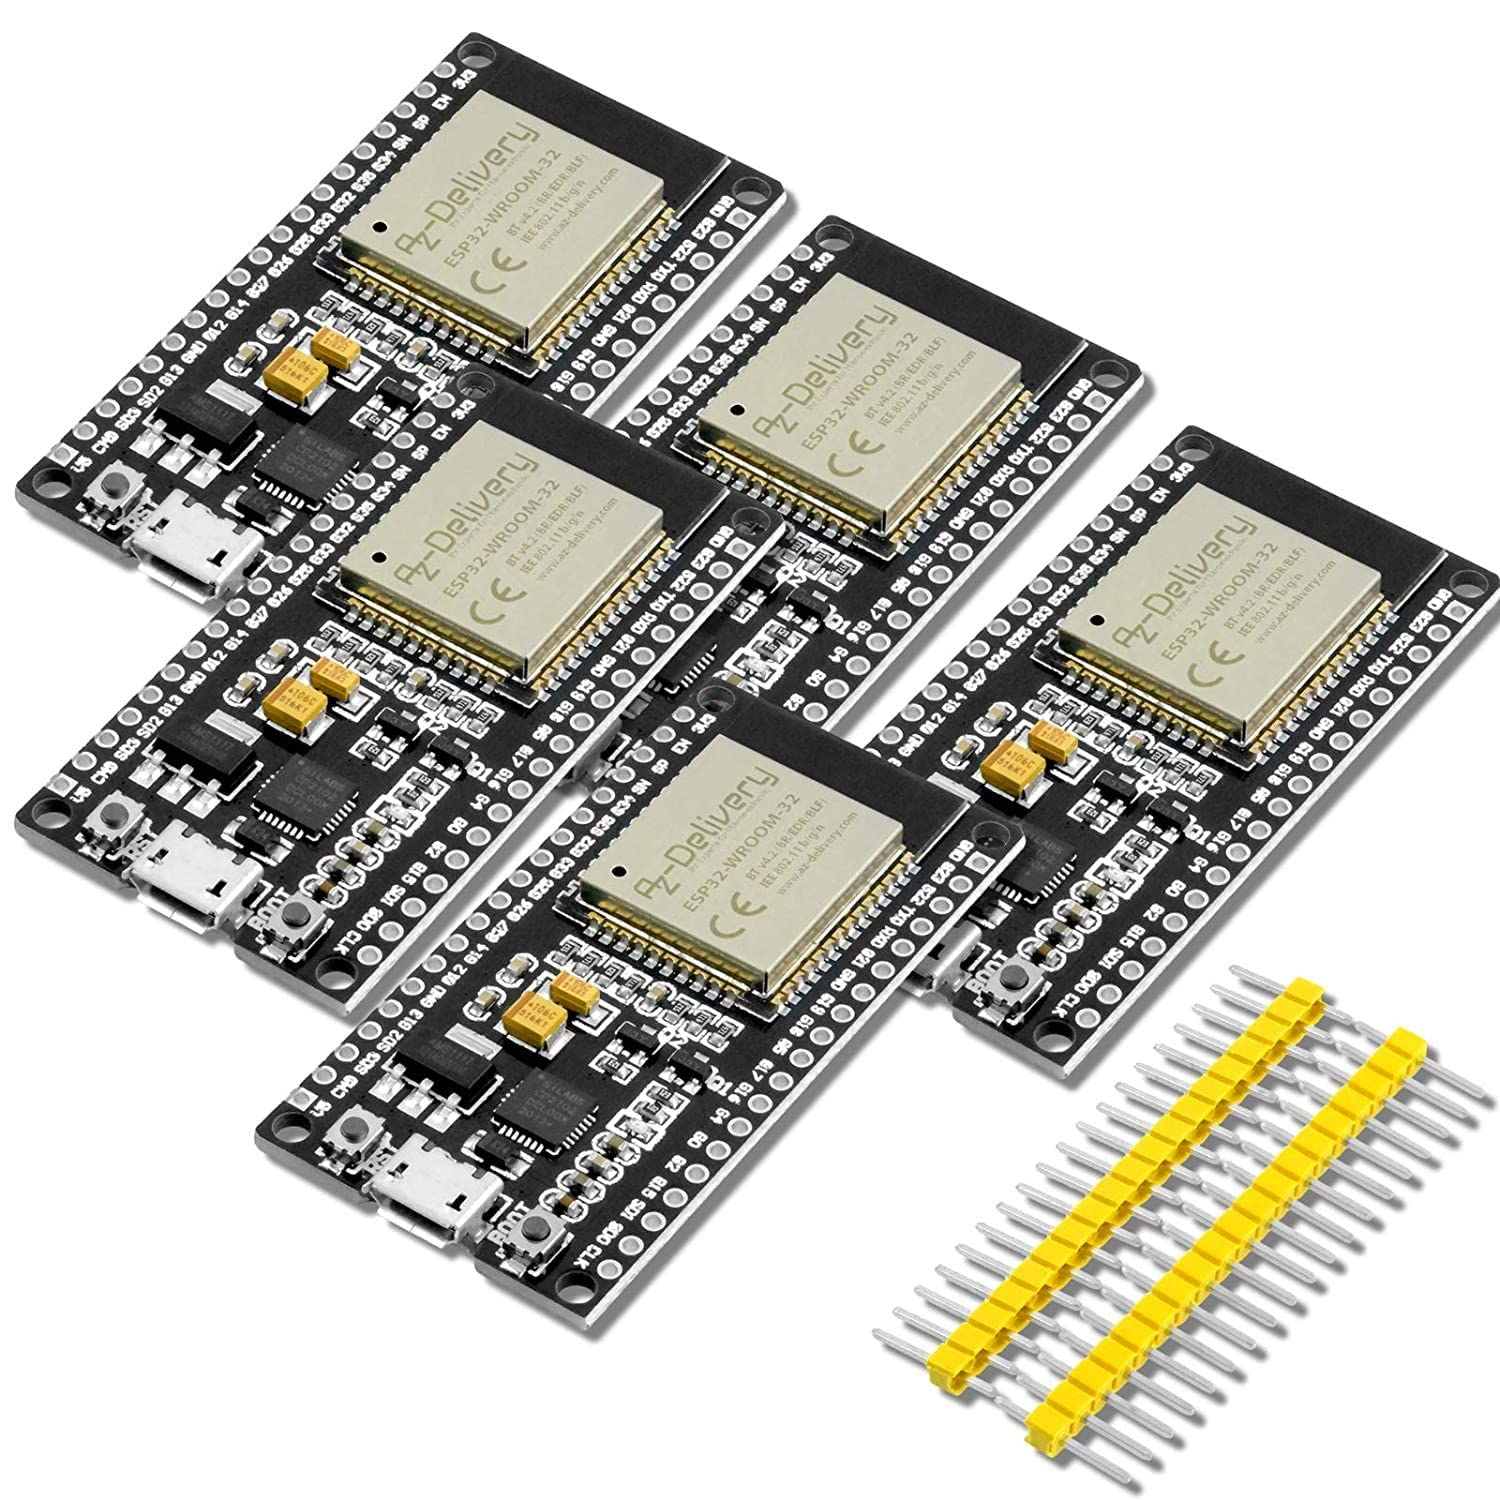
\includegraphics[width=0.5\textwidth]{material/esp-32-dev-board-c.jpg}
%            
\includegraphics[width=0.5\textwidth]{material/lora-sx1278.jpg}
            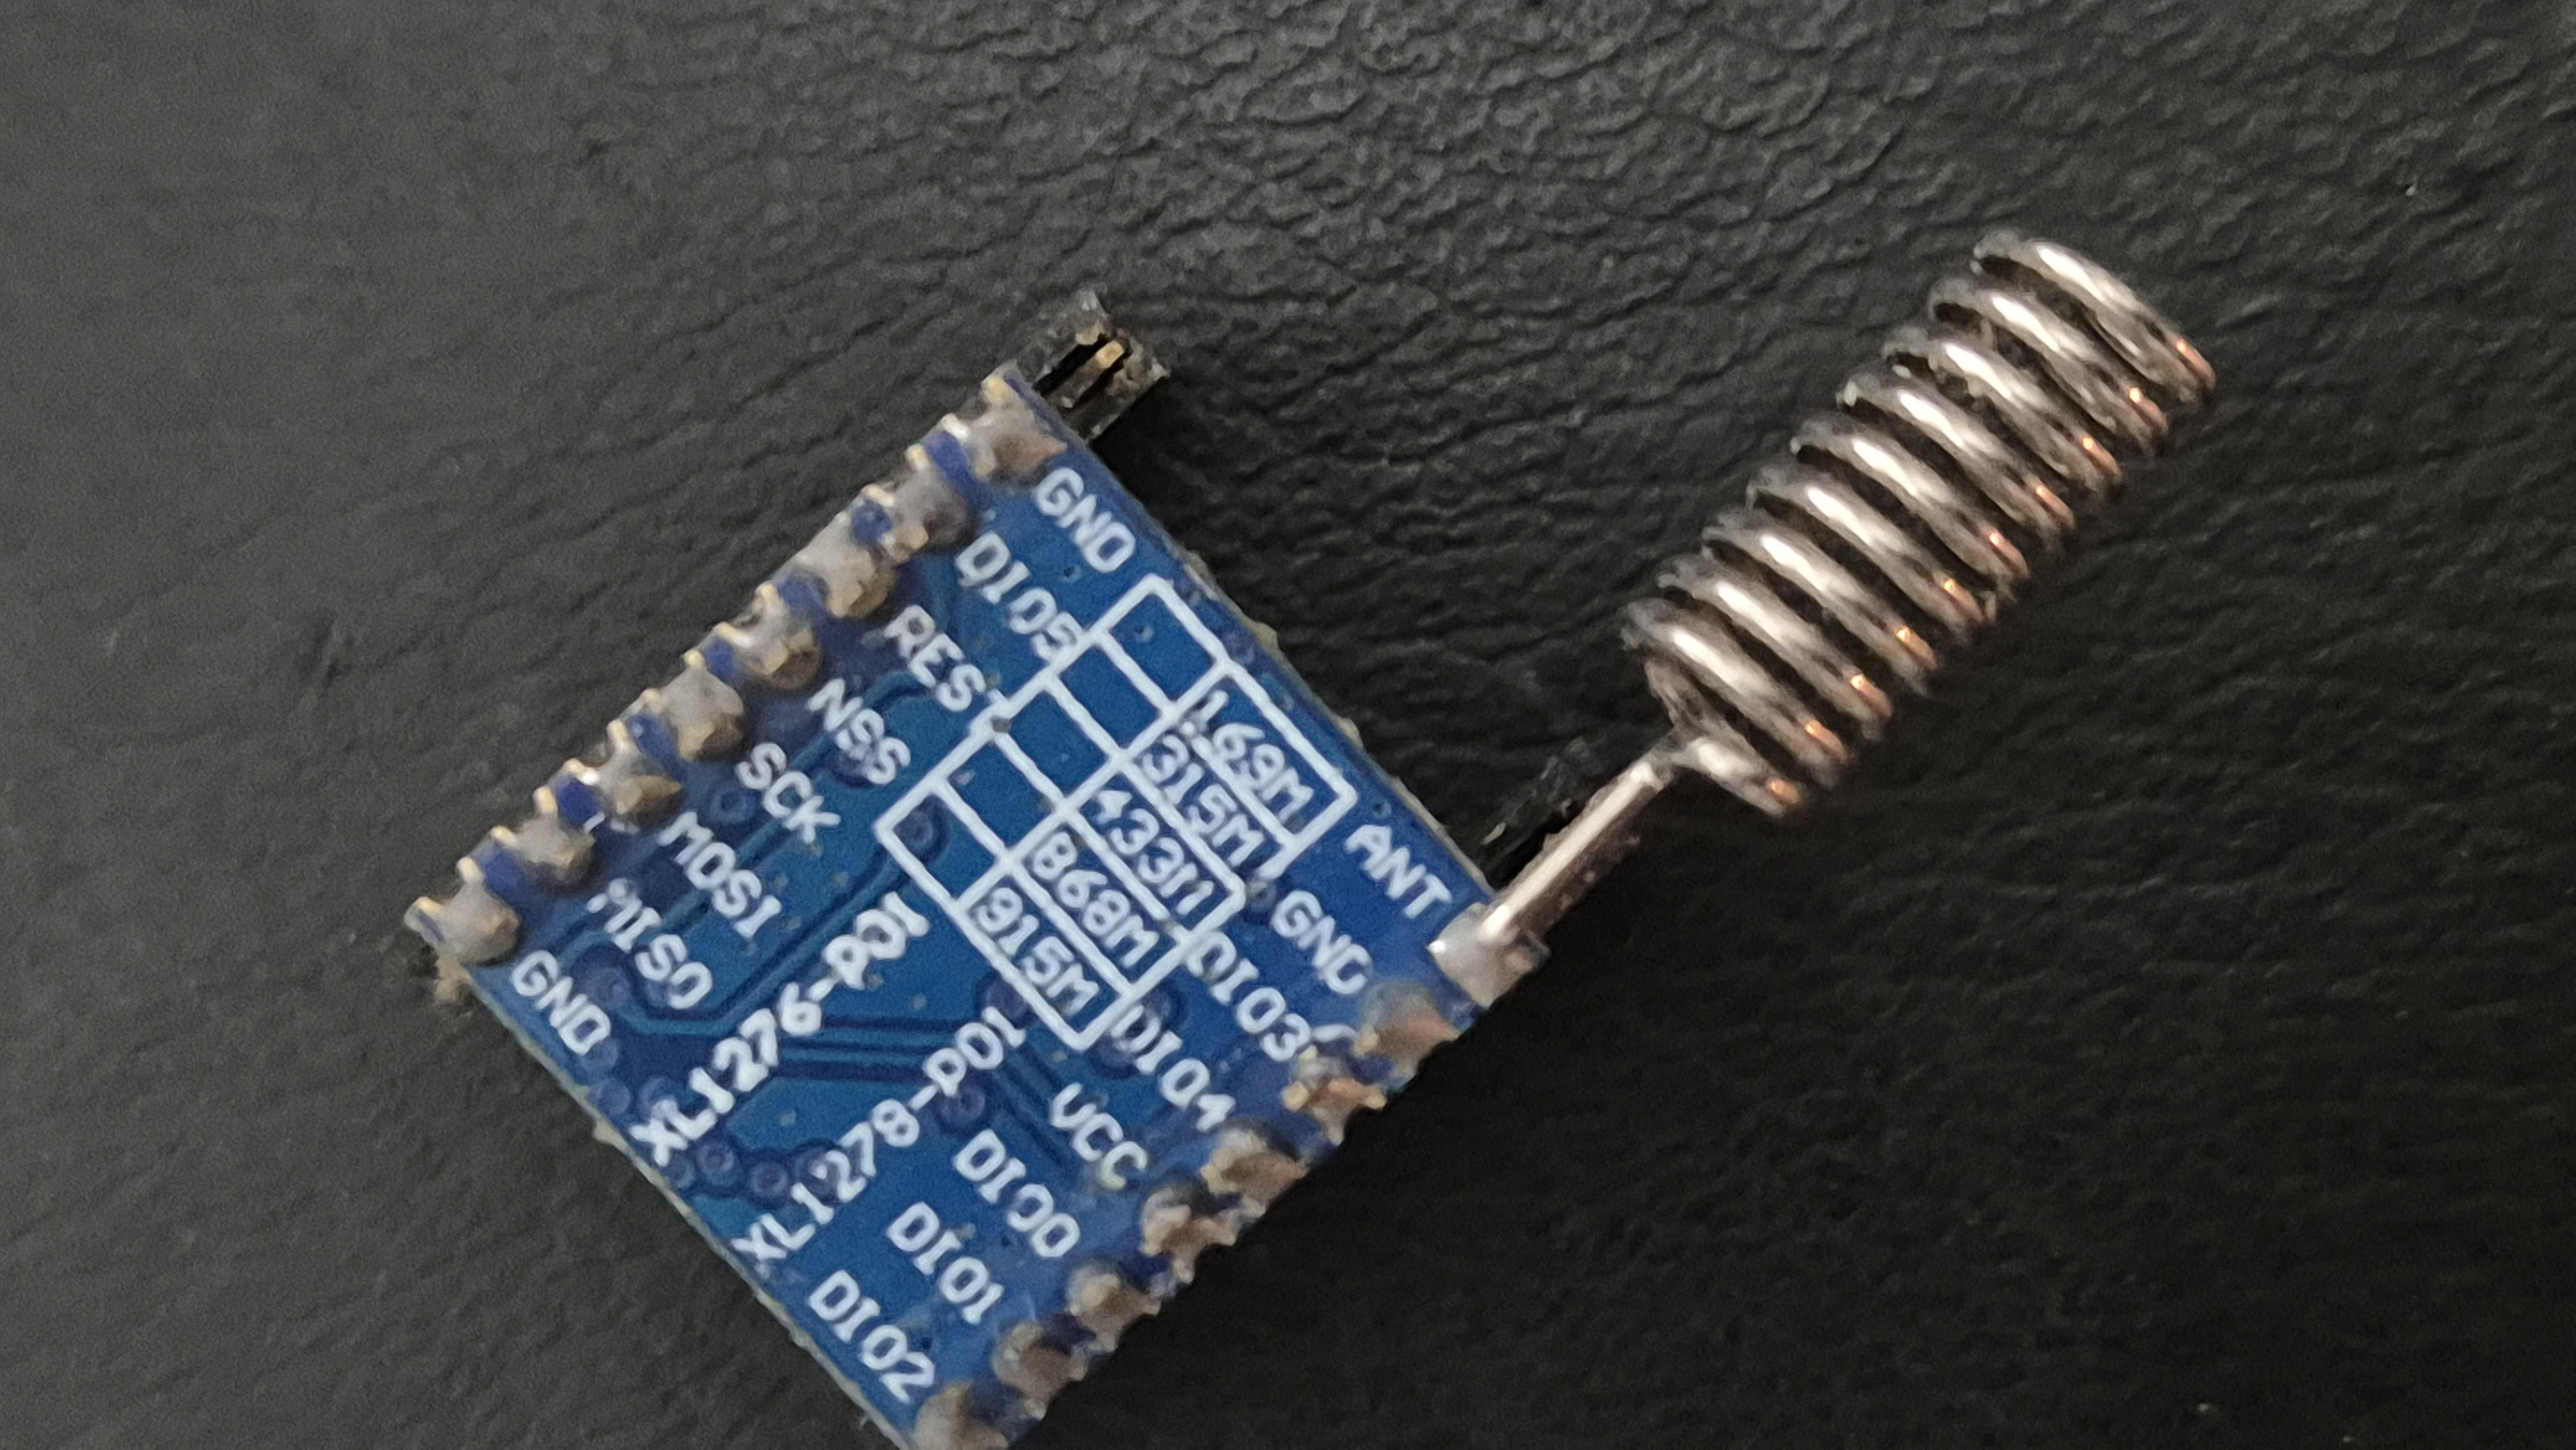
\includegraphics[width=0.5\textwidth]{material/sx1278.jpg}
        \end{center}
    \end{column}
\end{columns}
\begin{itemize}
    \item Based on an \alert{ESP-32 Development Board}.
    \item LoRa Transceiver: \alert{SX1278}.
    \item Programmed via the \alert{Arduino IDE} or \alert{PlatformIO}.
    \item No sensor is connected -- currently it's just a prove of concept.
\end{itemize}
\end{frame}
